\documentclass[t,10pt,fleqn]{beamer}

%%% My preferred theme choices.  More information is available at
%
%  https://en.wikipedia.org/wiki/Beamer_(LaTeX)
%  http://mirrors.ctan.org/macros/latex/contrib/beamer/doc/beameruserguide.pdf

\usetheme{Malmoe}
\usecolortheme{rose}
\useinnertheme{rounded}
\useoutertheme[subsection=false,footline=authorinstitute]{miniframes}
\usenavigationsymbolstemplate{}

%%% The following command inserts a slide with the outline at the
%%% beginning of each section, highlighting the current section.  It
%%% is optional.

\AtBeginSection[]
{
  \begin{frame}{Outline}
    \tableofcontents[currentsection]
  \end{frame}
}

\newenvironment{amatrix}[1]{%
  \left(\begin{array}{@{}*{#1}{r}|r@{}}
}{%
  \end{array}\right)
}

\newenvironment{bulletlist}
   {
      \begin{list}
         {$\bullet$}
%         {$\cdot$}
         {
            \setlength{\itemsep}{.5ex}
            \setlength{\parsep}{0ex}
            \setlength{\leftmargin}{1.5 em}
            \setlength{\rightmargin}{0.5em}
            \setlength{\parskip}{0ex}
            \setlength{\topsep}{0ex}
         }
   }
   {
      \end{list}
   }


\newcount\arrowcount
\newcommand\arrows[1]{
        \global\arrowcount#1
        \ifnum\arrowcount>0
                \begin{matrix}
                \expandafter\nextarrow
        \fi
}

\newcommand\nextarrow[1]{
        \global\advance\arrowcount-1
        \ifx\relax#1\relax\else \xrightarrow{#1}\fi
        \ifnum\arrowcount=0
                \end{matrix}
        \else
                \\
                \expandafter\nextarrow
        \fi
}


%%% It is sometimes easier to have graphics in a subfolder (or
%%% subfolders) of the current folder, in this case that folder is
%%% called Figures
\graphicspath{ 
  {Figures/}
}


\usepackage{multicol}
  \usepackage{booktabs}
  \usepackage{amsmath}
\usepackage{epsfig}
\usepackage{enumerate}

\def\ds{\displaystyle}
\def\u{{\mathbf u}}
\def\v{{\mathbf v}}
\def\w{{\mathbf w}}

\def\A{{\mathbf A}}



\def\B{{\mathbf B}}
\def\C{{\mathbf C}}
\def\D{{\mathbf D}}
\def\E{{\mathbf E}}
\def\X{{\mathbf X}}
\def\U{{\mathbf U}}

\def\T{{\mathbf T}}

\def\det{\text{det}}
\def\row{\text{row}}
\def\col{\text{col}}
\def\dim{\text{dim}}
\def\span{\text{span}}
\def\rank{\text{rank}}
\def\dom{\text{dom}}
\def\domain{\text{domain}}
\def\range{\text{range}}
\def\RREF{\text{RREF}}
\def\null{\text{null}}
\def\nullity{\text{nullity}}
\def\ker{\text{ker}}


\def\e{{\mathbf e}}
\def\x{{\mathbf x}}
\def\y{{\mathbf y}}
\def\b{{\mathbf b}}
\def\c{{\mathbf c}}

\def\r{{\mathbf r}}

\def\0{{\mathbf 0}}
\def\v{{\mathbf v}}
\def\I{{\mathbf I}}


\def\AA{\mathcal{A}}
\def\R{\mathcal{R}}

\def\S{\mathcal{S}}

\def\V{\mathcal{V}}

\def\M{\mathcal{M}}

\def\({\biggr ( }
\def\){\biggr ) }

\def\[{\biggr [ }
\def\]{\biggr ] }

\def\d{\partial}

\newcommand{\tu}[1]{\underline{\textit{#1}}}

% This is the main file
% This is the main file

\title[Reaction-Diffusion Equations]%
      {Data-driven Comparison of Plague Models}
\subtitle{Senior Project}
\author[Luke Mattfeld]{Luke Mattfeld}
\institute[EWU]{Eastern Washington University}
\date{Fall, 2020}

\begin{document}

\begin{frame}
\titlepage

\end{frame}
%-------------------------------------------------------------------------------------------------------------------------------------
%-------------------------------------------------------------------------------------------------------------------------------------
\section{Background}
%------------------------------------------------------------------------------------------------------------------------------
\begin{frame}{Patterns}
\vspace{-.3cm}
\begin{block}{Pattern Formation}
  \begin{itemize}
    \pause
    \item Patterns in Nature:
    \pause
    \\
    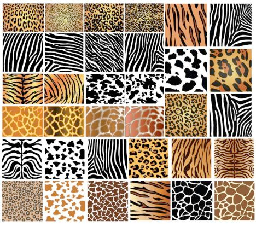
\includegraphics[width=0.5\textwidth]{creature_patterns2.png}
  \end{itemize}
\end{block}
\pause
\end{frame}

\begin{frame}{Simpler Model}
  \vspace{-.3cm}
  \begin{block}{Morphogenesis}
    \begin{itemize}
      \pause
      \item Morphogens related to cell growth
      \pause
      \item Chemical that react
      \pause
      \item Chemicals that diffuse?
      \pause
    \end{itemize}
  \end{block}
  \pause
  \end{frame}


%-------------------------------------------------------------------------------------------------------------------------------------
%-------------------------------------------------------------------------------------------------------------------------------------
\section{Preliminary Models}
%------------------------------------------------------------------------------------------------------------------------------
\begin{frame}{Pneumonic Model}
  \vspace{-.3cm}
  \begin{block}{General Model}
      $$\frac{\partial A}{\partial t} = F(A,B) + D_{A} \nabla A$$
      $$\frac{\partial B}{\partial t} = G(A,B) + D_{B} \nabla B$$
      \pause
    \begin{itemize}
      \item A, B Concentration of Chemical Morphogens
      \pause
      \item $F, G$ Chemical Reaction Equations
      \pause
      \item $D_{A}, D_{B}$ Diffusion coefficients
      \pause
      \item $\nabla A$, $\nabla B$ Diffusion
      \pause
    \end{itemize}
  \end{block}
  \pause
\end{frame}

\begin{frame}{Keeling-Gilligan Rat Model}
  \vspace{-.3cm}
  \begin{block}{Turing-specific models}
    \begin{itemize}
      \item Reaction Diffusion is very general
      \pause
      \item Most RD equations don't form patterns
      \pause
    \end{itemize}
      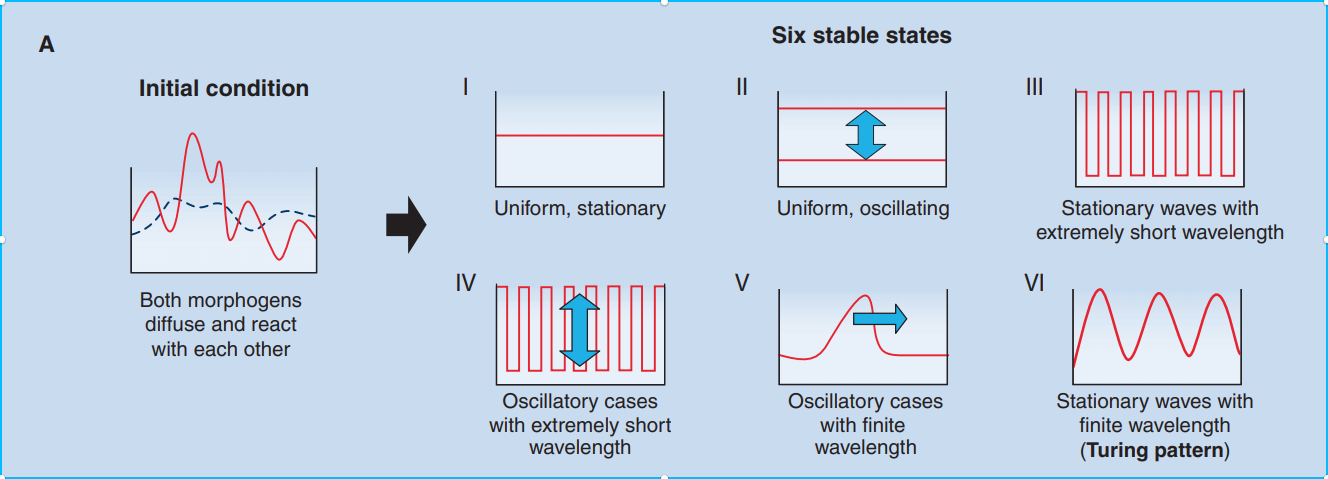
\includegraphics[width=0.75\textwidth]{stable_states.png}\\
      \pause
      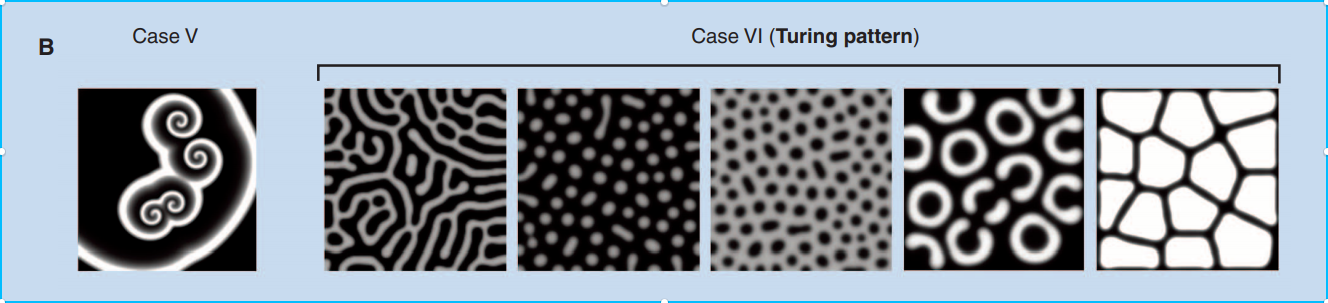
\includegraphics[width=0.75\textwidth]{turing_pattern.png}
  \end{block}
  \pause
  \begin{block}{Diagram}
    \begin{itemize}
      \item Reaction Diffusion is very general
      \pause
      \item Most RD equations don't form patterns
      \pause
    \end{itemize}
      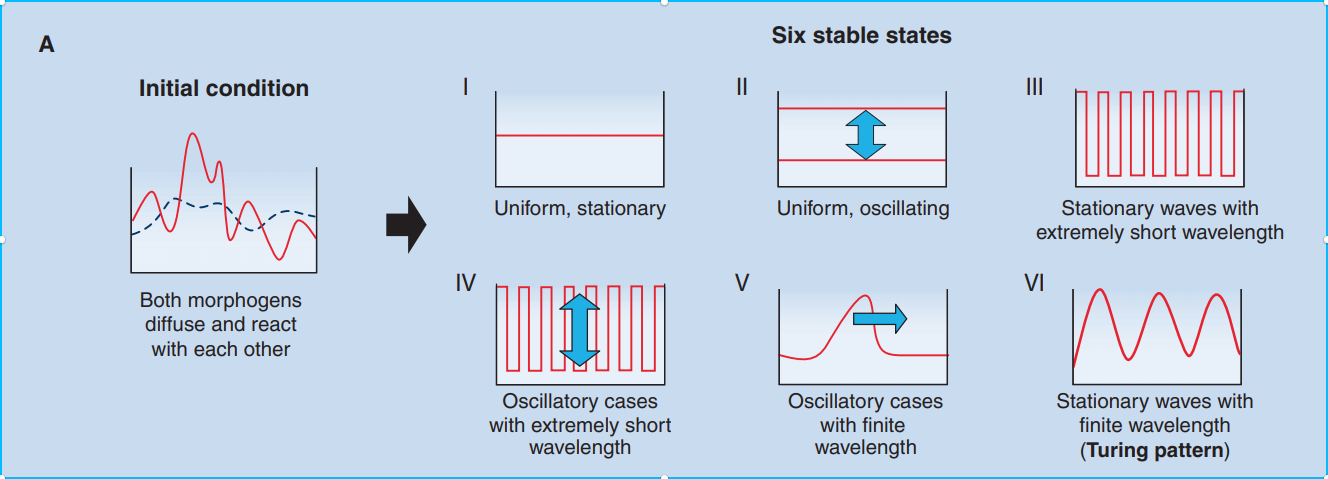
\includegraphics[width=0.75\textwidth]{stable_states.png}\\
      \pause
      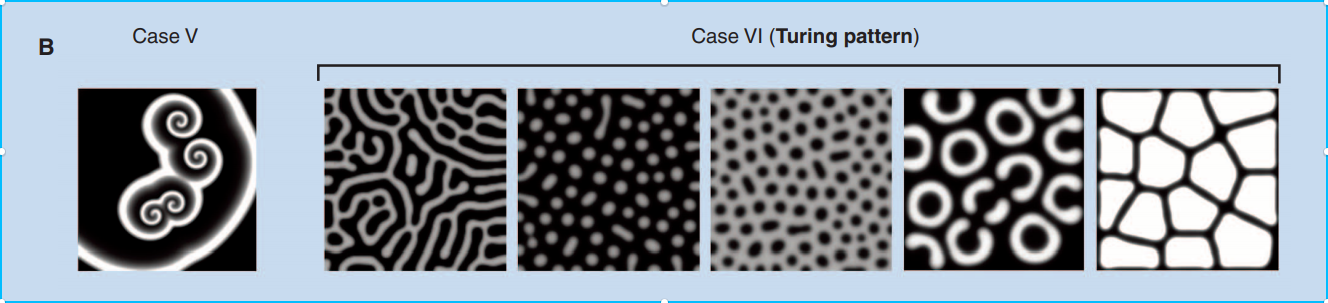
\includegraphics[width=0.75\textwidth]{turing_pattern.png}
  \end{block}
  \pause
\end{frame}

\begin{frame}{Lynch-Oster Rat Model}
  \vspace{-.3cm}
  \begin{block}{Turing-specific models}
    \begin{itemize}
      \item Reaction Diffusion is very general
      \pause
      \item Most RD equations don't form patterns
      \pause
    \end{itemize}
      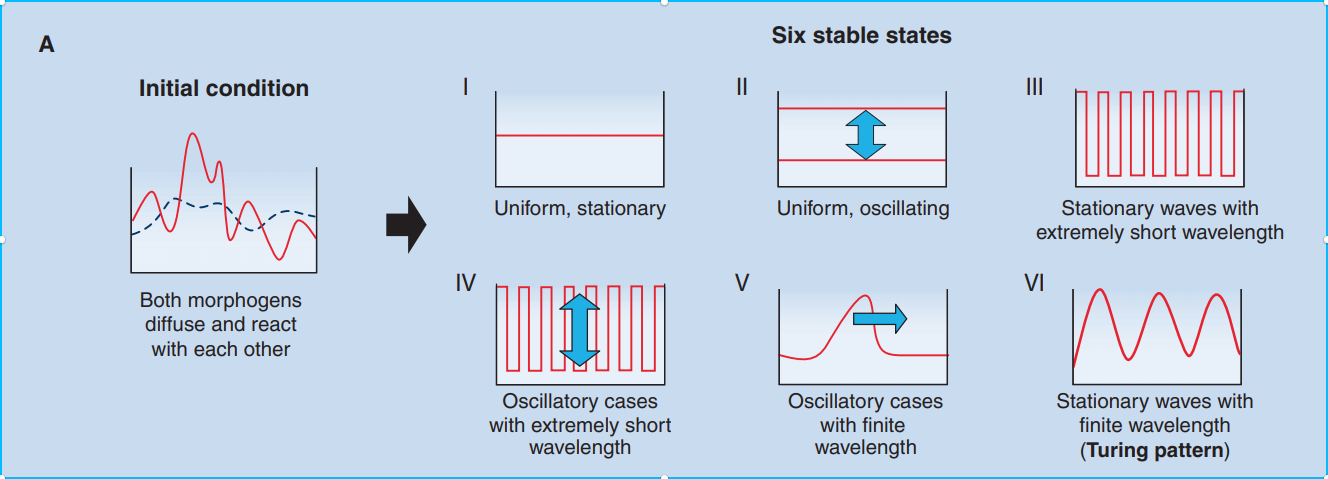
\includegraphics[width=0.75\textwidth]{stable_states.png}\\
      \pause
      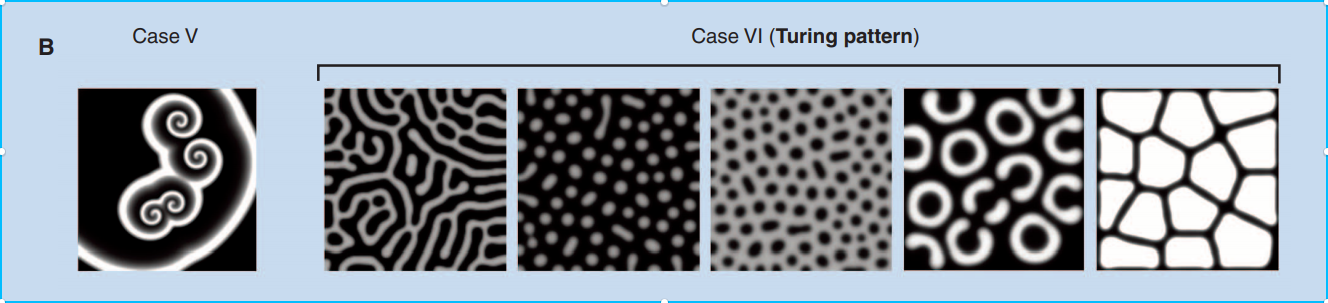
\includegraphics[width=0.75\textwidth]{turing_pattern.png}
  \end{block}
  \pause
\end{frame}

\begin{frame}{Human-Ectoparasite Model}
  \vspace{-.3cm}
  \begin{block}{Turing-specific models}
    \begin{itemize}
      \item Reaction Diffusion is very general
      \pause
      \item Most RD equations don't form patterns
      \pause
    \end{itemize}
      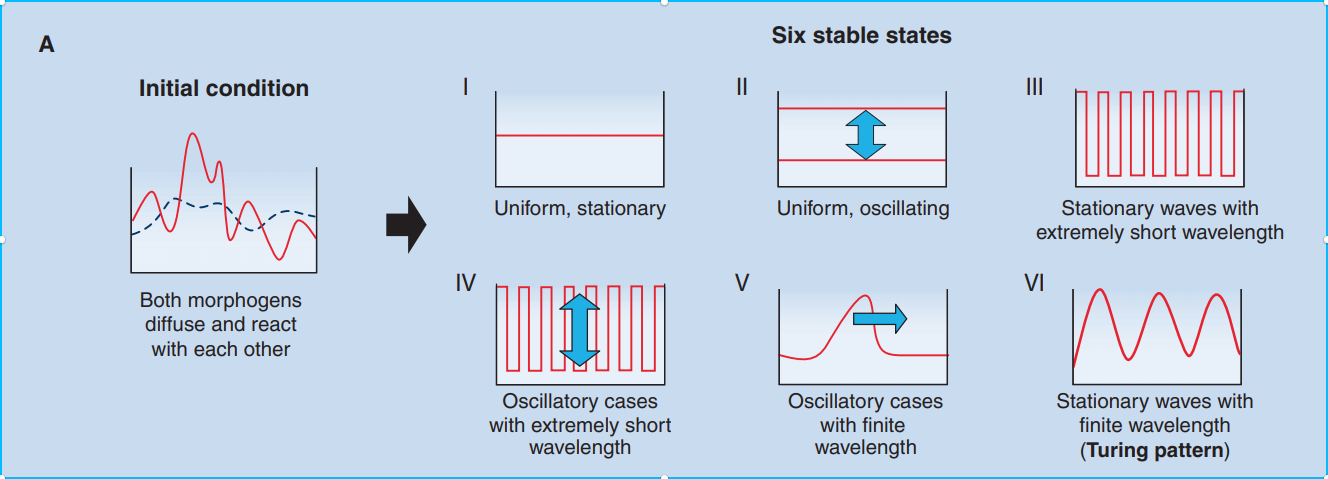
\includegraphics[width=0.75\textwidth]{stable_states.png}\\
      \pause
      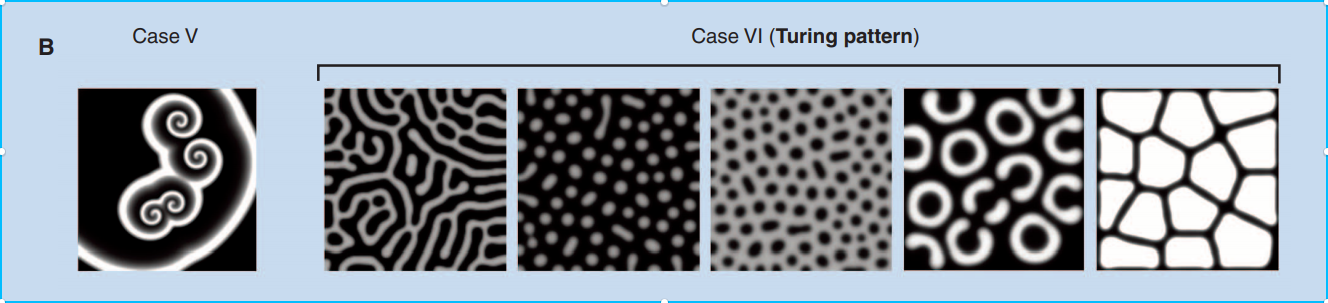
\includegraphics[width=0.75\textwidth]{turing_pattern.png}
  \end{block}
  \pause
\end{frame}


%-------------------------------------------------------------------------------------------------------------------------------------
%-------------------------------------------------------------------------------------------------------------------------------------
\section{Method: MCMC}
%------------------------------------------------------------------------------------------------------------------------------
\begin{frame}{Method}
\vspace{-.3cm}
\begin{block}{Markov Chains}
  \begin{itemize}
    \pause
    \item Patterns in Nature:
    \pause
    \\
    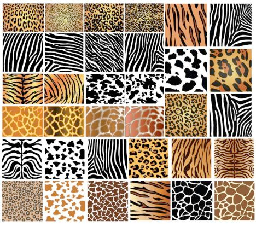
\includegraphics[width=0.5\textwidth]{creature_patterns2.png}
  \end{itemize}
\end{block}
\pause
\end{frame}

\begin{frame}{Method}
  \vspace{-.3cm}
  \begin{block}{Monte Carlo Method}
    \begin{itemize}
      \pause
      \item Morphogens related to cell growth
      \pause
      \item Chemical that react
      \pause
      \item Chemicals that diffuse?
      \pause
    \end{itemize}
 \end{block}
\pause
\end{frame}


\begin{frame}{Method}
\vspace{-.3cm}
\begin{block}{MCMC}
  \begin{itemize}
    \pause
    \item Patterns in Nature:
    \pause
    \\
    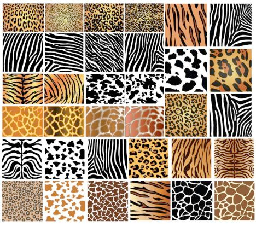
\includegraphics[width=0.5\textwidth]{creature_patterns2.png}
  \end{itemize}
\end{block}
\pause
\end{frame}
  
  
%-------------------------------------------------------------------------------------------------------------------------------------
%-------------------------------------------------------------------------------------------------------------------------------------
\section{Comparison}
%------------------------------------------------------------------------------------------------------------------------------
\begin{frame}{Patterns}
\vspace{-.3cm}
\begin{block}{Pattern Formation}
  \begin{itemize}
    \pause
    \item Patterns in Nature:
    \pause
    \\
    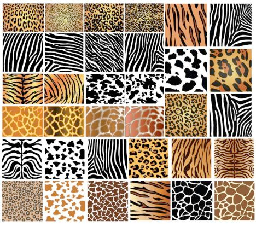
\includegraphics[width=0.5\textwidth]{creature_patterns2.png}
  \end{itemize}
\end{block}
\pause
\end{frame}



%-------------------------------------------------------------------------------------------------------------------------------------
%-------------------------------------------------------------------------------------------------------------------------------------
\section{Results}
%------------------------------------------------------------------------------------------------------------------------------
\begin{frame}{Patterns}
\vspace{-.3cm}
\begin{block}{Pattern Formation}
  \begin{itemize}
    \pause
    \item Patterns in Nature:
    \pause
    \\
    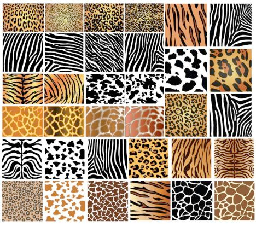
\includegraphics[width=0.5\textwidth]{creature_patterns2.png}
  \end{itemize}
\end{block}
\pause
\end{frame}

\begin{frame}{Simpler Model}
  \vspace{-.3cm}
  \begin{block}{Morphogenesis}
    \begin{itemize}
      \pause
      \item Morphogens related to cell growth
      \pause
      \item Chemical that react
      \pause
      \item Chemicals that diffuse?
      \pause
    \end{itemize}
  \end{block}
  \pause
  \end{frame}



%-------------------------------------------------------------------------------------------------------------------------------------
%-------------------------------------------------------------------------------------------------------------------------------------
\section{Future Work}
%------------------------------------------------------------------------------------------------------------------------------
\begin{frame}{Patterns}
\vspace{-.3cm}
\begin{block}{Pattern Formation}
  \begin{itemize}
    \pause
    \item Patterns in Nature:
    \pause
    \\
    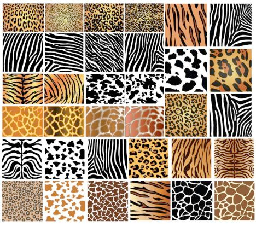
\includegraphics[width=0.5\textwidth]{creature_patterns2.png}
  \end{itemize}
\end{block}
\pause
\end{frame}

\begin{frame}{Future Testbed}
\vspace{-.3cm}
\begin{block}{Pattern Formation}
  \begin{itemize}
    \pause
    \item Patterns in Nature:
    \pause
    \\
    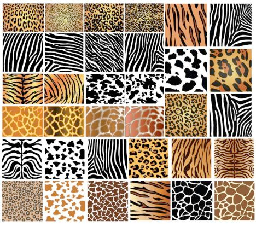
\includegraphics[width=0.5\textwidth]{creature_patterns2.png}
  \end{itemize}
\end{block}
\pause
\end{frame}


\end{document}


